
%(BEGIN_QUESTION)
% Copyright 2010, Tony R. Kuphaldt, released under the Creative Commons Attribution License (v 1.0)
% This means you may do almost anything with this work of mine, so long as you give me proper credit

Tre designere diskuterer beste måte å installere en {\it varmeveksler} for varmeutveksling mellom to fluider. Én sier at fluidene bør gå i motsatt retning (``contra-flow''). Den andre sier de bør gå i samme retning. Den tredje sier det ikke spiller noen rolle:

$$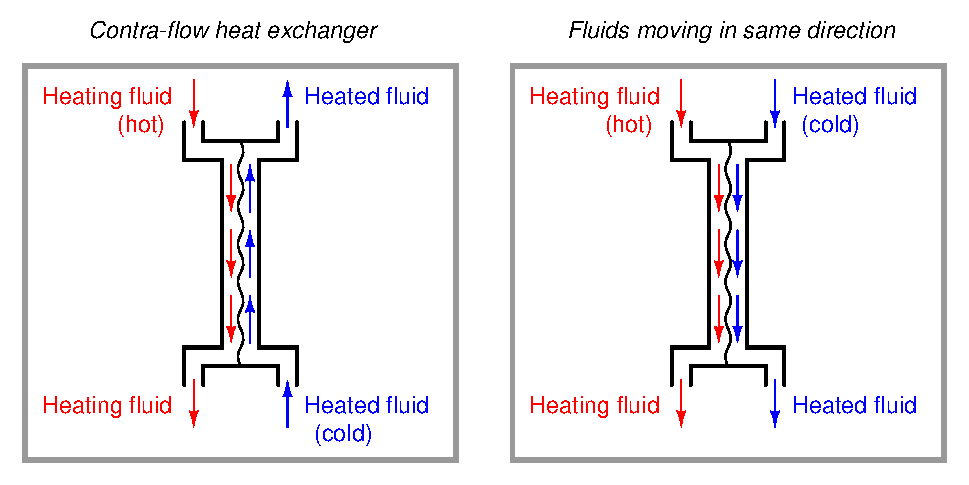
\includegraphics[width=15.5cm]{i00610x01.eps}$$

Identifiser først hvilken av de tre som har rett.

\vskip 10pt

Vurder deretter om {\it lengden} på vekslerne er relevant. Hvis begge vekslerne gjøres like mye lengre, vil dette favorisere én strømningstype (motstrøm versus samme retning)?

\vskip 10pt

Forklar begrunnelsen for begge svarene dine, med henvisning til relevante termodynamiske prinsipper.

\underbar{file i00610}
%(END_QUESTION)





%(BEGIN_ANSWER)

Motstrøm (contra-flow) er best, uavhengig av vekslerlengde.

Grunnen er at motstrøm maksimerer temperaturdifferansen mellom varmende og oppvarmet fluid langs hele vekslerlengden. Dette er enklest å se ved tenkt uendelig lang veksler: i samme-retning-design vil fluidene utjevnes til en temperatur mellom innløpstemperaturene; i motstrøm kan de i prinsippet gå ut med temperatur nær den andre fluidets innløp.

\vskip 10pt

3 poeng for første svar, 3 poeng for andre svar. 4 poeng for korrekt forklaring (forutsatt at de to første svarene er riktige).

%(END_ANSWER)





%(BEGIN_NOTES)

{\bf Dette spørsmålet er ment for eksamen og ikke arbeidsark!}.

%(END_NOTES)

